\section{Schallgeschwindigkeit}

\subsection{Arbeitsgrundlagen}

Die Schallgeschwindigkeit $c$ kann mit der Formel
\begin{equation}
    c=\frac{s}{t}
    \label{eq:schallgeschwindigkeit}
\end{equation}
berechnet werden, wobei $s$ die Messstrecke ist und $t$ die Laufzeit.


\subsection{Durchf\"{u}hrung}

\subsubsection*{Versuchsanordnung}

Zur Bestimmung der Schallgeschwindigkeit wurde die Laufzeit eines Schallpulses \"{u}ber eine Strecke
der L\"{a}nge $s = (2.561 \pm 0.003) m$ mehrfach gemessen (die gesch\"{a}tzte Unsicherheit der Strecke $\pm 3 mm$
kommt daher, dass die genaue Lage der Mikrophon-Membran nicht festgestellt werden konnte). Die
Temperatur im Experimentierraum betrug $\vartheta=23 \degree C$.


\subsubsection*{Messergebnisse}

Die gemessene Gr\"ossen sind in der Tabelle \ref{table:schallgeschwindigkeit} ersichtlich.

\begin{center}
    \begin{threeparttable}
        \caption{Gemessene Gr\"ossen}
        \begin{tabular}{cccc}
            \toprule
            Messung & Laufzeit $t_i$ & Messung & Laufzeit $t_i$ \\
            \midrule
            1  & 7.59 & 11 & 7.40 \\
            2  & 7.16 & 12 & 7.58 \\
            3  & 6.97 & 13 & 7.04 \\
            4  & 7.55 & 14 & 7.17 \\
            5  & 6.77 & 15 & 6.89 \\
            6  & 6.97 & 16 & 7.20 \\
            7  & 7.74 & 17 & 7.33 \\
            8  & 7.18 & 18 & 7.21 \\
            9  & 7.32 & 19 & 8.05 \\
            10 & 7.70 & 20 & 7.63 \\
           \bottomrule
        \end{tabular}
        \begin{tablenotes}
            \small
            \item \textbf{Hinweis:} Daten wurden vom Auftragsdokument kopiert.
        \end{tablenotes}
        \label{table:schallgeschwindigkeit}
    \end{threeparttable}
\end{center}

Es soll die mitlere Laufzeit $\bar{t}$ sowie die Schallgeschwindigkeit $c$ (mitsammt Fehler) ermittelt werden.


\subsubsection*{Mittlere Laufzeit}

Die mittlere Laufzeit wird berechnet mit
\begin{equation}
    \bar{t} = \frac{1}{20} \sum_{i=1}^{20} t_i = \frac{7.59+7.16+6.97+7.55+6.77+\ldots}{20} = \SI{7.32}{\milli\second}
\end{equation}

Die Standardabweichung wird berechnet mit
\begin{equation}
    s_t = \sqrt{ \frac{ \sum_{i=1}^{20} (t_i - \bar{t})^2 }{20-1} } = 0.33
\end{equation}

und der Fehler mit
\begin{equation}
    s_{\bar{t}} = \frac{s_t}{\sqrt{20}} = \SI{0.07}{\milli\second}
\end{equation}

Somit ergibt sich die mittlere Laufzeit mit Unsicherheit als $t = (7.32 \pm 0.07)\SI{}{\milli\second}$.

\subsubsection*{Schallgeschwindigkeit}

Die Schallgeschwindigkeit wird mit $c=\frac{s}{t}$ berechnet. Wir wissen dass
$s=\bar{s}+s_{\bar{s}}=(2.561\pm0.003) \textrm{m}$
und
$t=\bar{t}+s_{\bar{t}}=(7.32\pm0.07) \textrm{ms}$.

Da die Schallgeschwindigkeit eine Funktion von mehreren Messgr\"ossen ist, muss mit Hilfe der
Gauss'schen Fehlerfortpflanzungsgesetzes der Fehler berechnet werden. Dazu wird die Formel $c=\frac{s}{t}$
partitiell abgeleitet nach $s$ und $t$
\begin{equation}
	\frac{\partial c}{\partial s} = \frac{1}{t} \textrm{\hspace{10mm} und \hspace{10mm}} \frac{\partial c}{\partial{t}} = \frac{-s}{t^2}
\end{equation}
und in die Formel des Fehlerfortpflanzungsgesetzes eingesetzt

\begin{equation}
	s_{\bar{c}} = \sqrt{\left(\frac{1}{t} \cdot s_{\bar{s}}\right)^2 + \left(\frac{-s}{t^2} \cdot s_{\bar{t}}\right)^2} = 3.5 \SI{}{\meter\per\second}
\end{equation}

Die mittlere Schallgeschwindigkeit berechnet sich mit
\begin{equation}
	\bar{c}=\frac{\bar{s}}{\bar{t}} = 349.7 \SI{}{\meter\per\second}
\end{equation}

Somit ergibt sich die Schallgeschwindigkeit
$c=(349.7 \pm 3.5) \SI{}{\meter\per\second}$


\subsubsection*{QtiPlot}

\begin{figure}[H]
    \center
    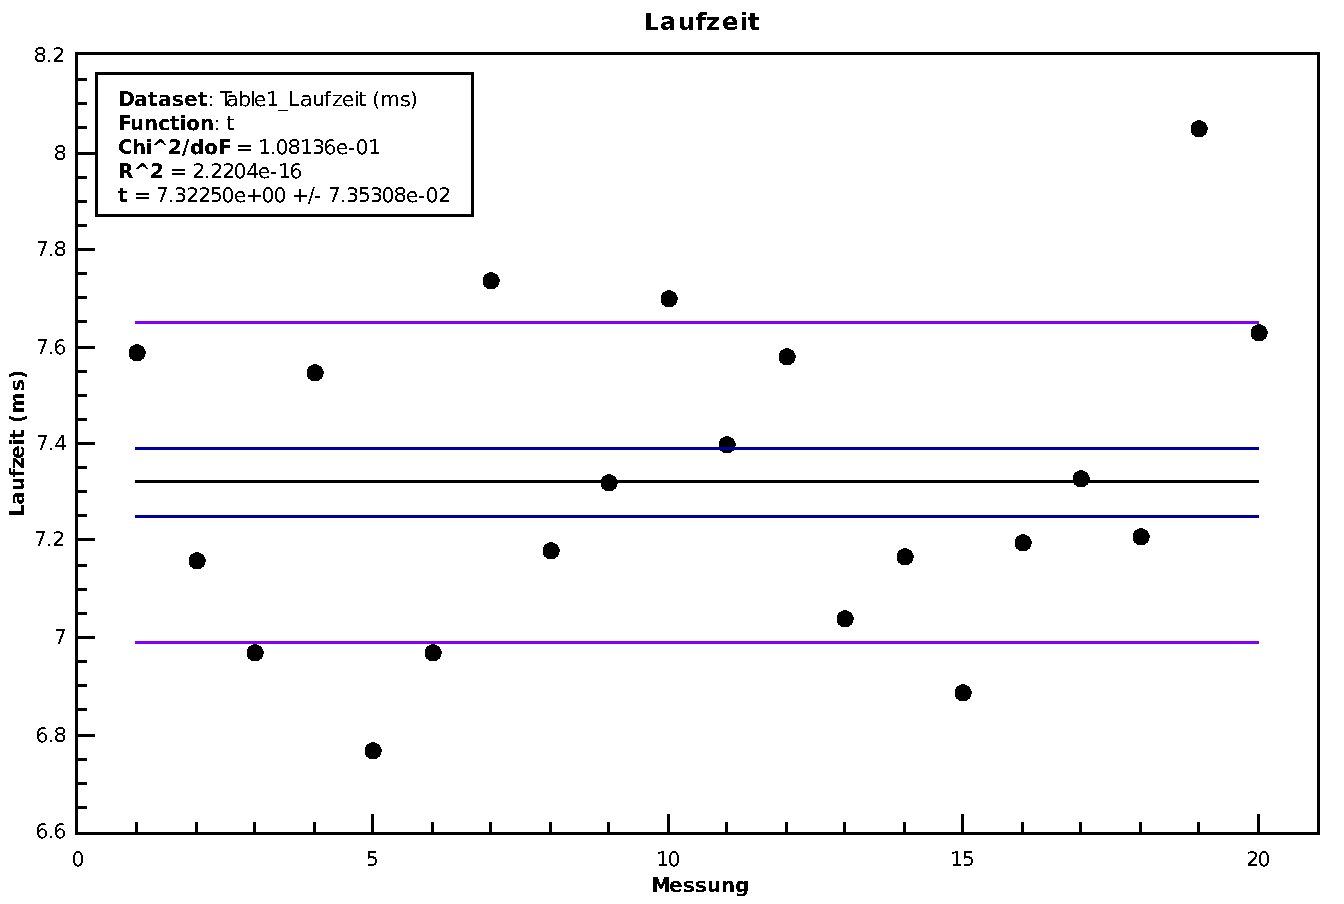
\includegraphics[width=.85\textwidth]{qtiplot/schallgeschwindigkeit}
    \caption{Visualisierung der Standardabweichung und Fehler}
    \label{fig:schallgeschwindigkeit}
\end{figure}

\subsection{Resultate und Diskussion}

Das Endresultat von $(347.7\pm2.9)\SI{}{\meter\per\second}$ ist ein wenig h\"oher als der
Literaturwert\footcite{ref:schallgeschwindigkeit} von $\SI{344}{\meter\per\second}$.
Warscheinlich liegt diese Abweichung daran, dass der Literaturwert bei $\vartheta=20\degree C$
auf Meeresh\"ohe gemessen wurde anstatt bei $\vartheta=23\degree C$ (und h\"ochstwarscheinlich
auf einer anderen H\"ohe). Die Schallgeschwindigkeit nimmt zu bei h\"oherem Temperatur.

